\documentclass[xcolor=dvipsnames,aspectratio=1610]{beamer}

\usepackage{graphicx}
\usepackage[scale=2]{ccicons}
\usepackage{multicol}
\usepackage[absolute,overlay]{textpos}
% \usepackage[texcoord,grid,gridunit=mm,gridcolor=red!10,subgridcolor=green!10]
% {eso-pic}

\newcommand{\exampleheight}{1.9cm}
\newcommand{\examplewidth}{16cm}

\usetheme[numbering=counter, progressbar=frametitle, sectionpage=none]{metropolis}
\setbeamercolor{background canvas}{bg=white}


\title{Conflict-Free Vertex Coloring of Planar Graphs}
\date{April 15, 2017}
\author{Shawn Seymour}

\begin{document}
  \maketitle

  \begin{frame}
    \begin{figure}[h]
      \centering
      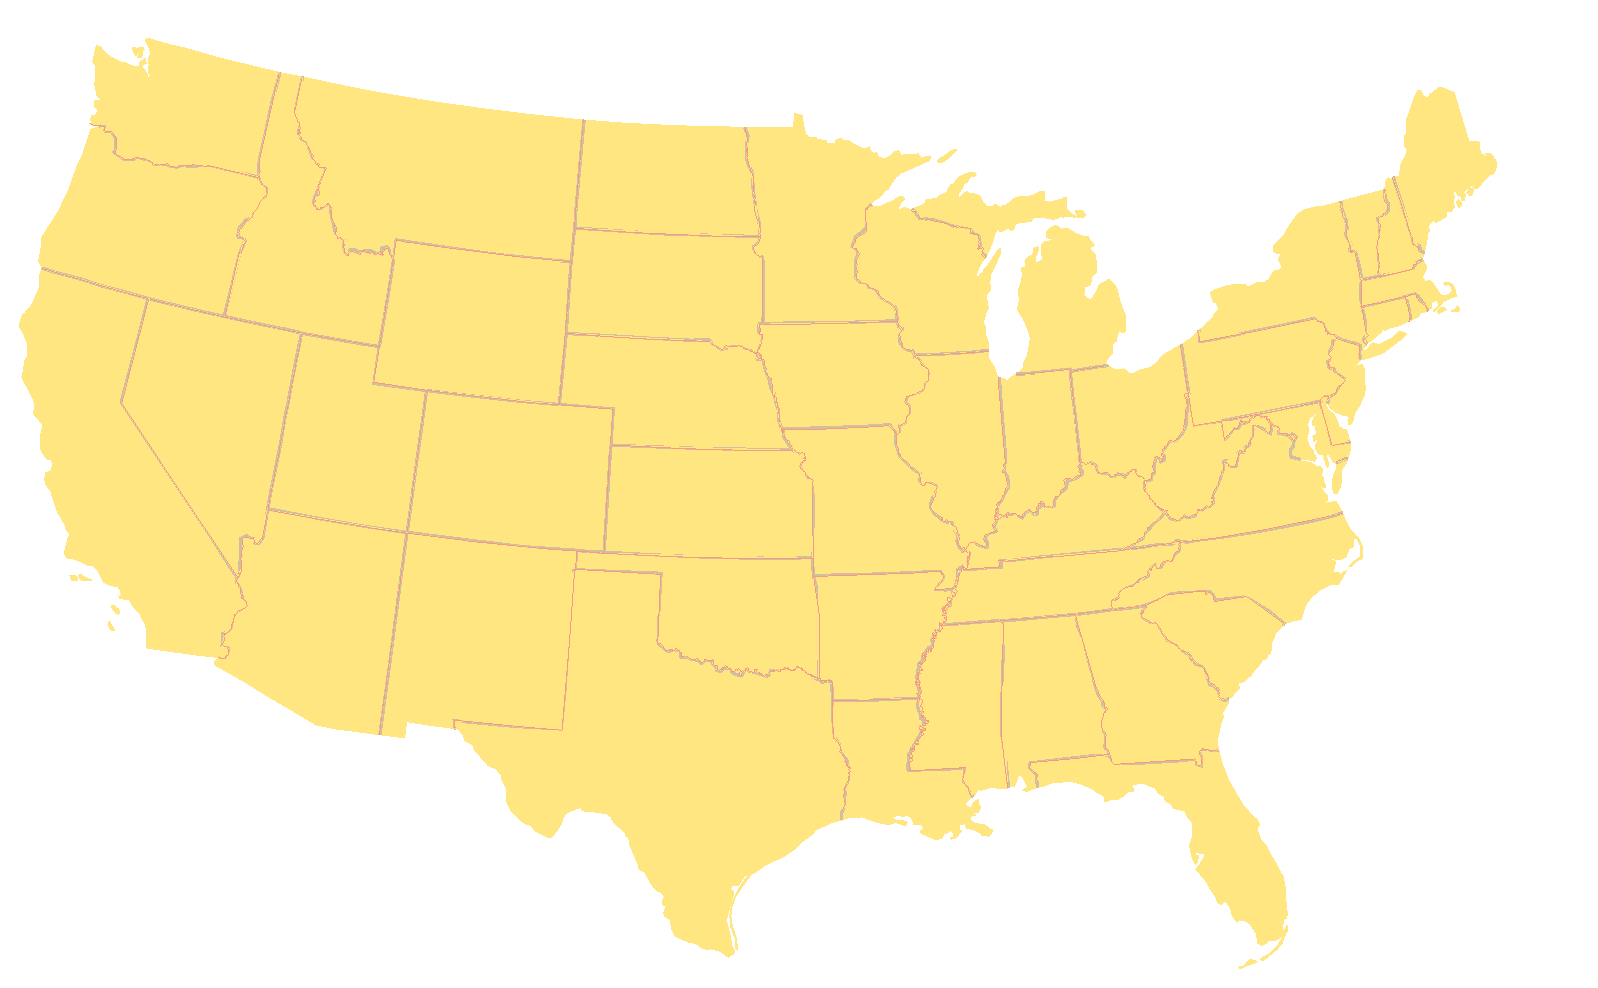
\includegraphics[width=14cm]{../figures/map-no-colors.pdf}
    \end{figure}
  \end{frame}

  \begin{frame}
    \begin{figure}[h]
      \centering
      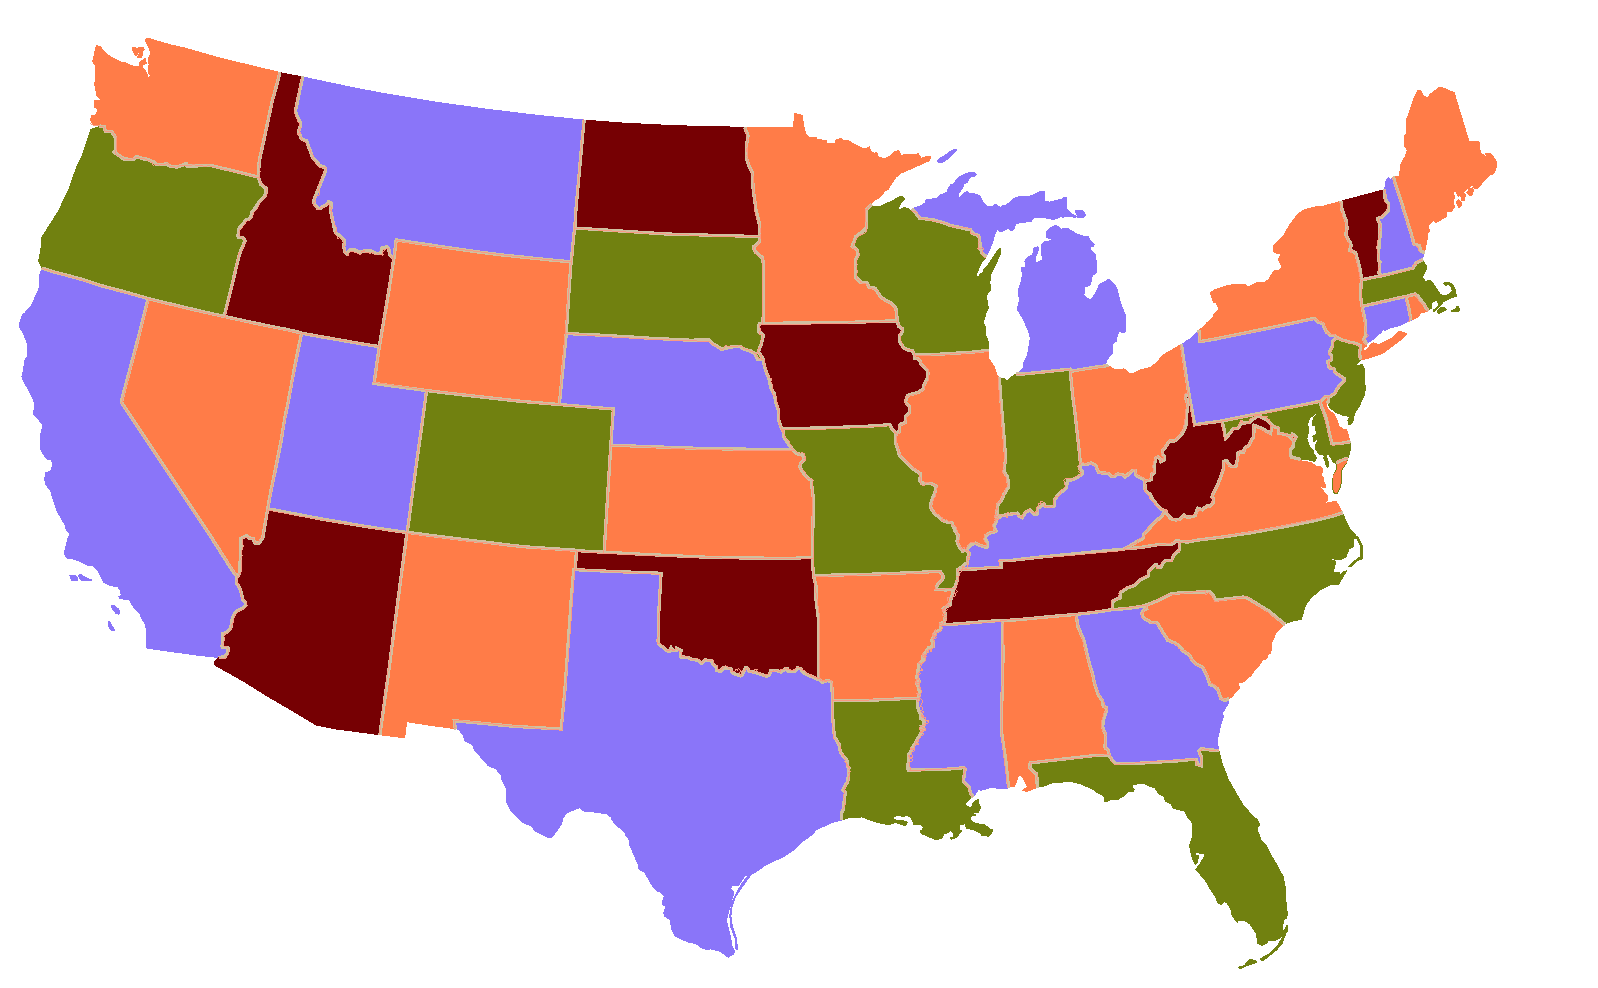
\includegraphics[width=14cm]{../figures/map-colors.pdf}
    \end{figure}
  \end{frame}

  \begin{frame}
    \frametitle{Overview}
    \begin{multicols}{2}
      \tableofcontents
    \end{multicols}
  \end{frame}

  \section{Background}

  \subsection{Graph Theory}

  \begin{frame}
    \frametitle{Graph Theory}



    \only<1-2>{
      \begin{textblock*}{\examplewidth}(0cm,\exampleheight) % {block width} (coords)
        \centering
        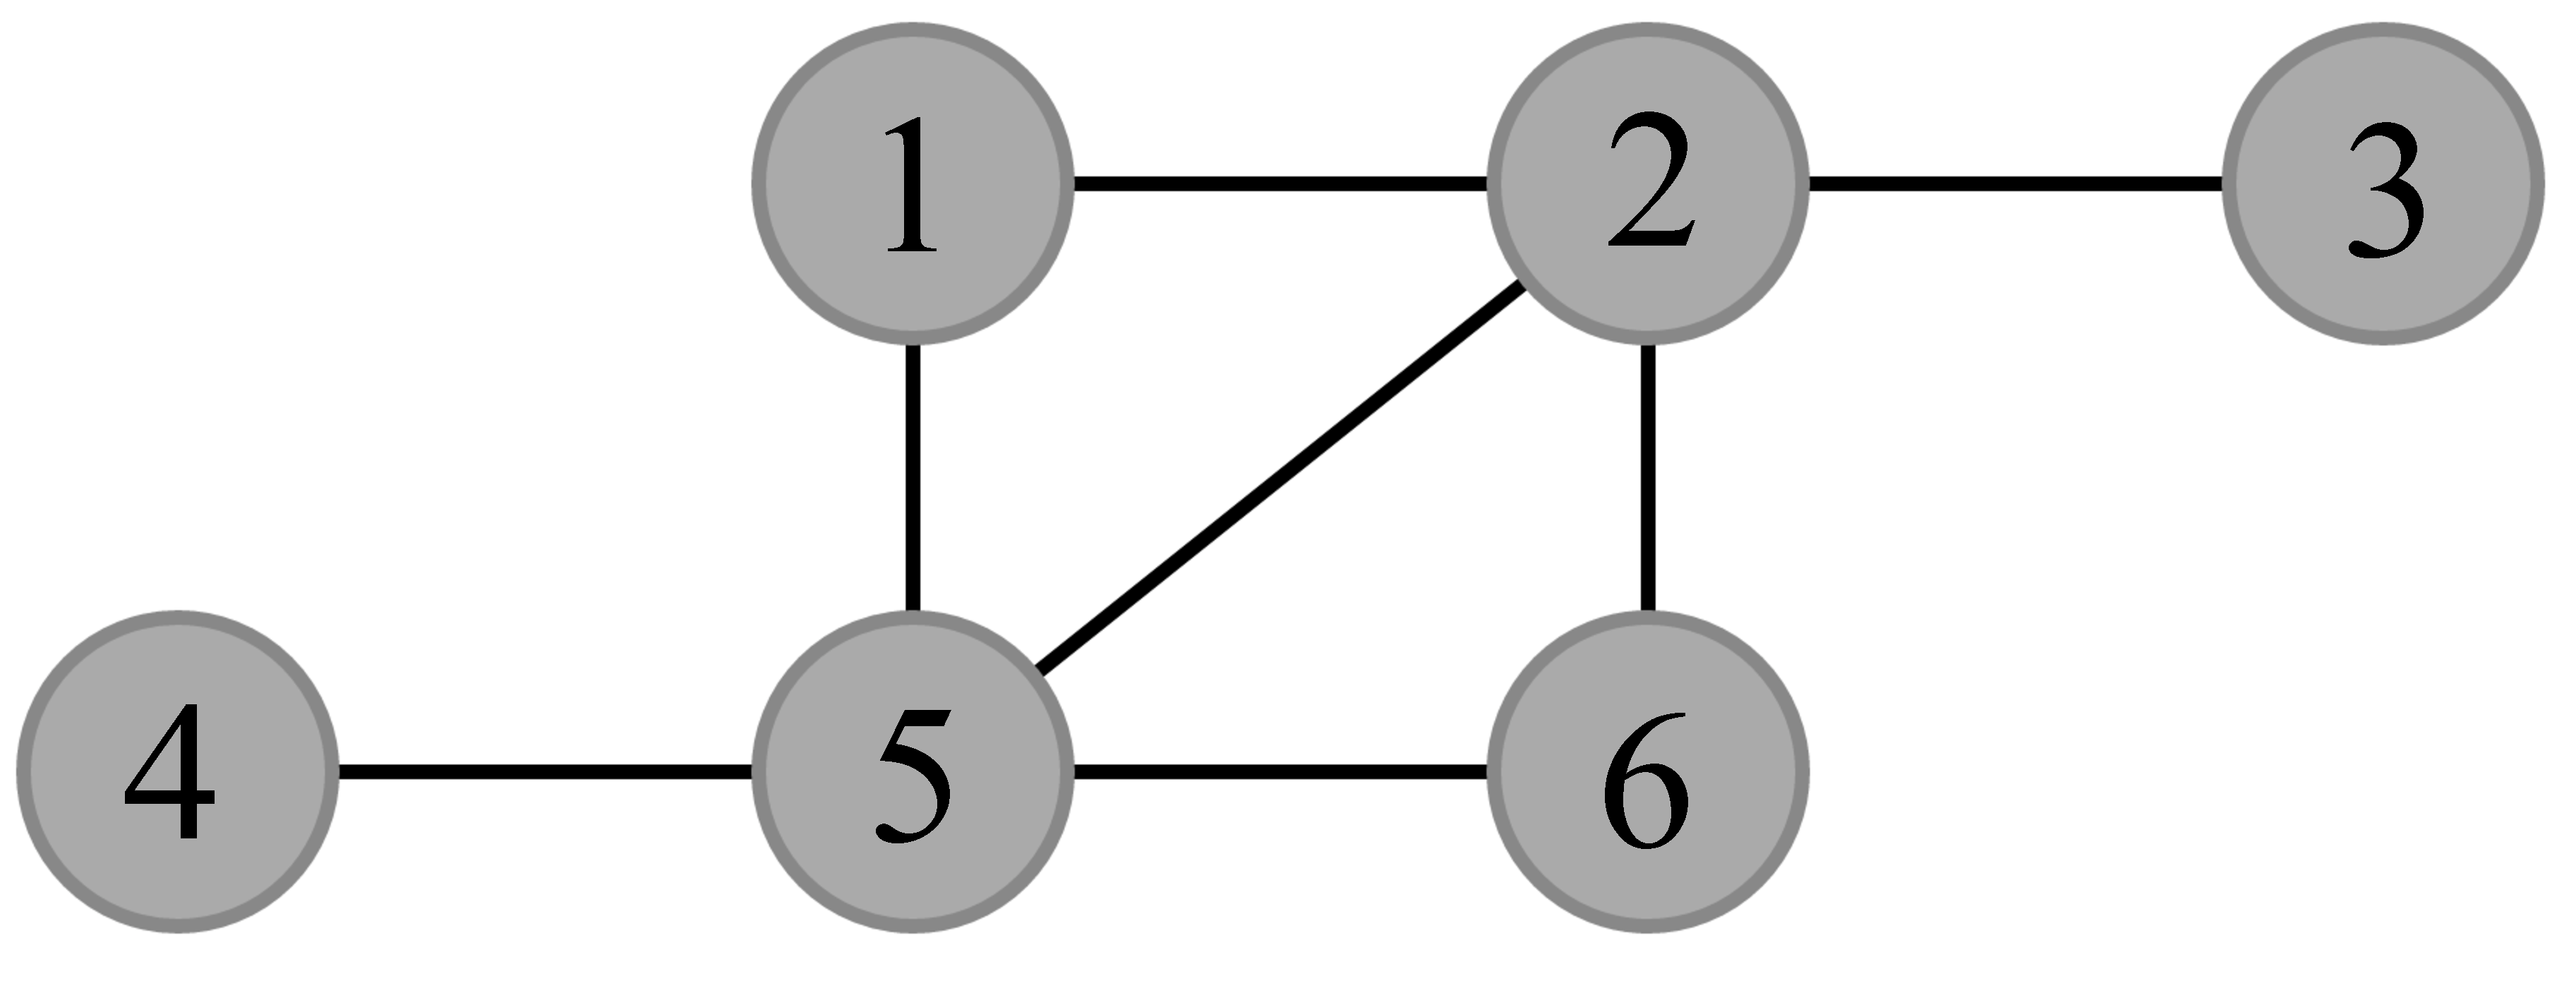
\includegraphics[width=8cm]{../figures/example.pdf}
      \end{textblock*}
    }

    \only<3> {
      \begin{textblock*}{\examplewidth}(0cm,\exampleheight) % {block width} (coords)
        \centering
        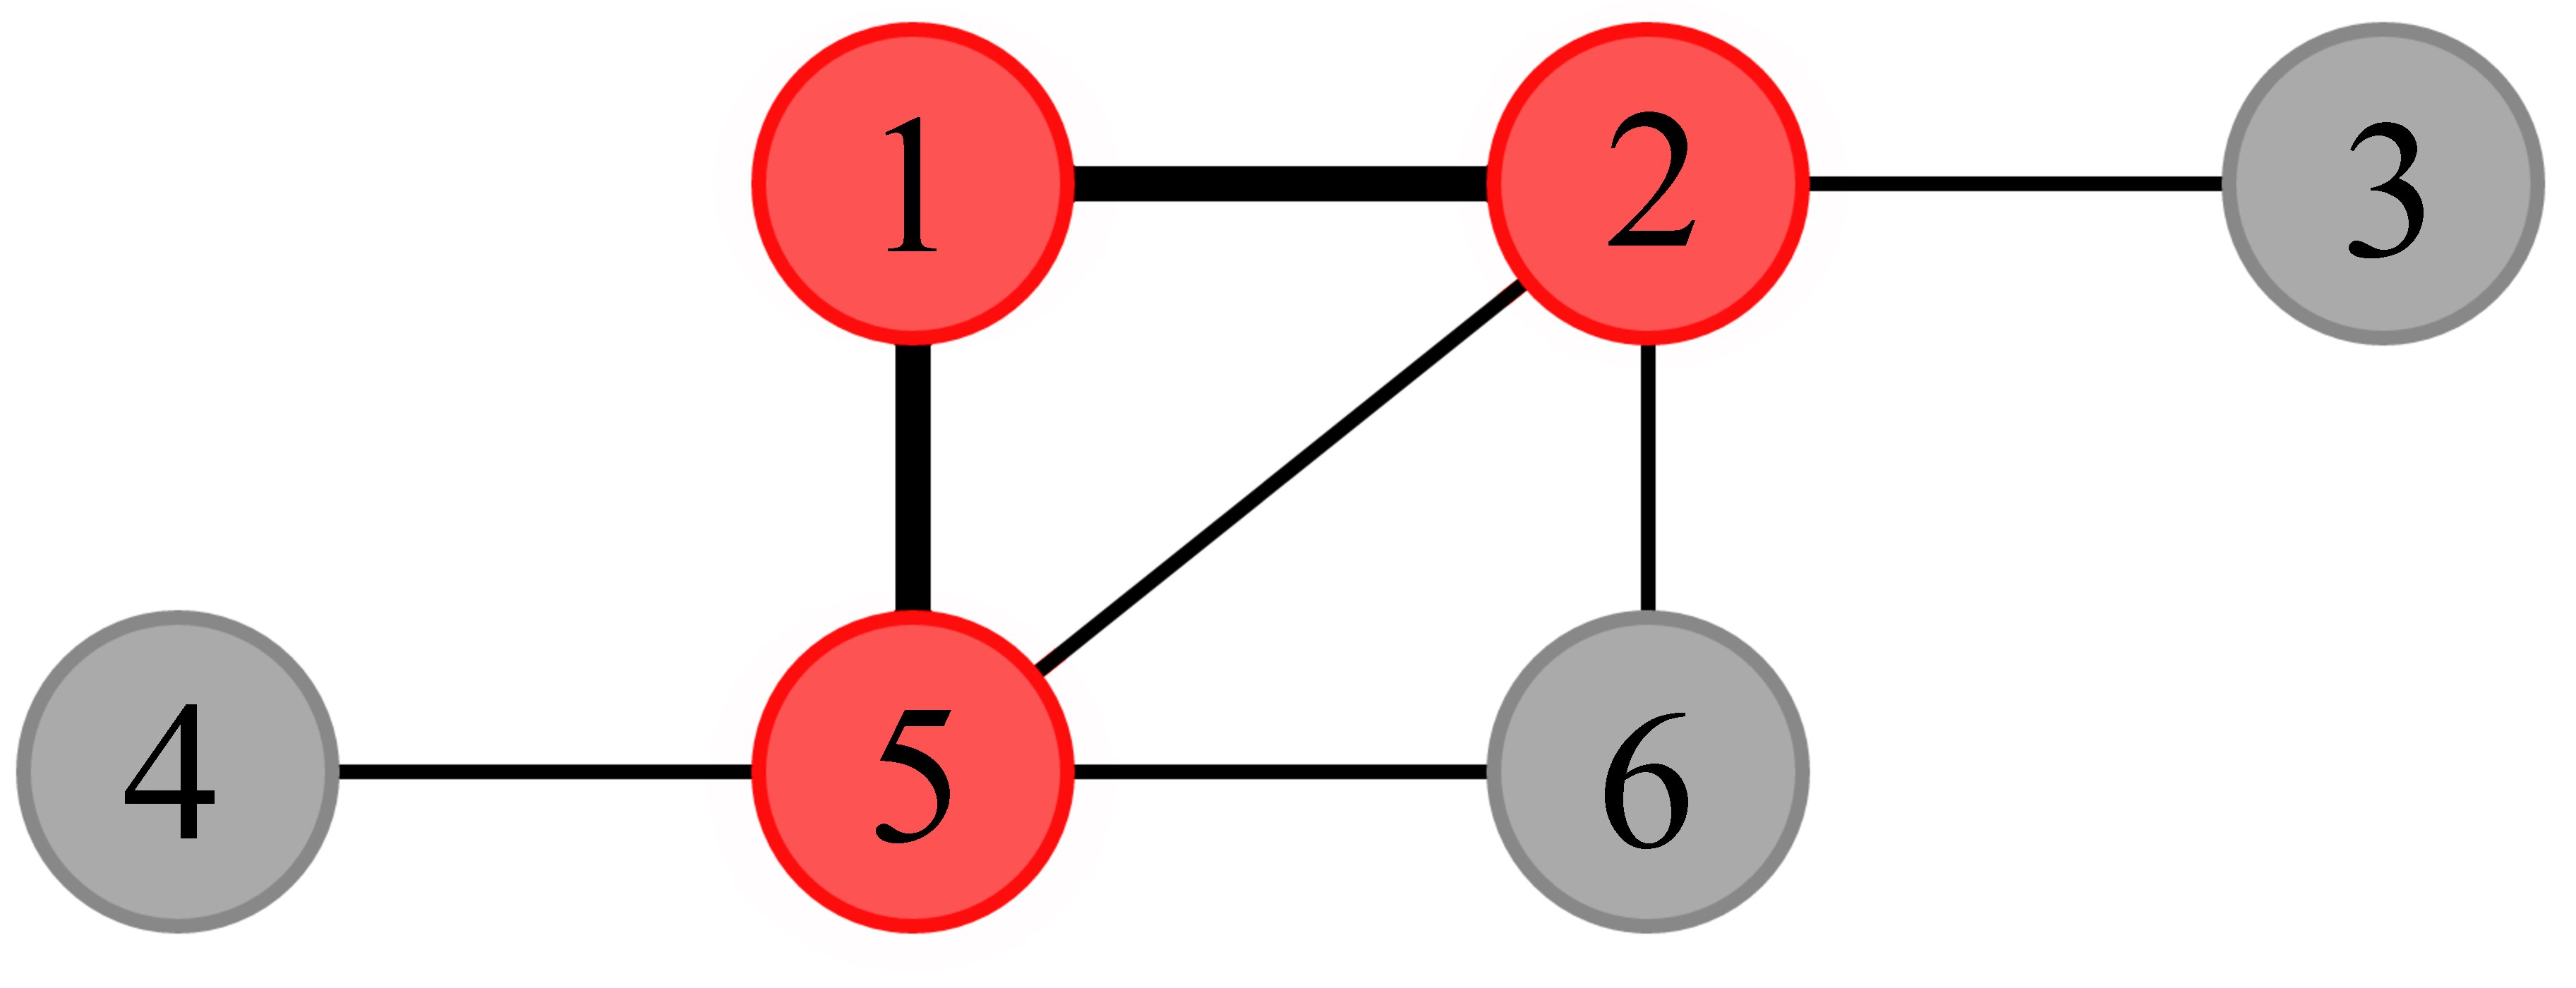
\includegraphics[width=8cm]{../figures/example-neighborhoods-1.pdf}
      \end{textblock*}
    }

    \only<4> {
      \begin{textblock*}{\examplewidth}(0cm,\exampleheight) % {block width} (coords)
        \centering
        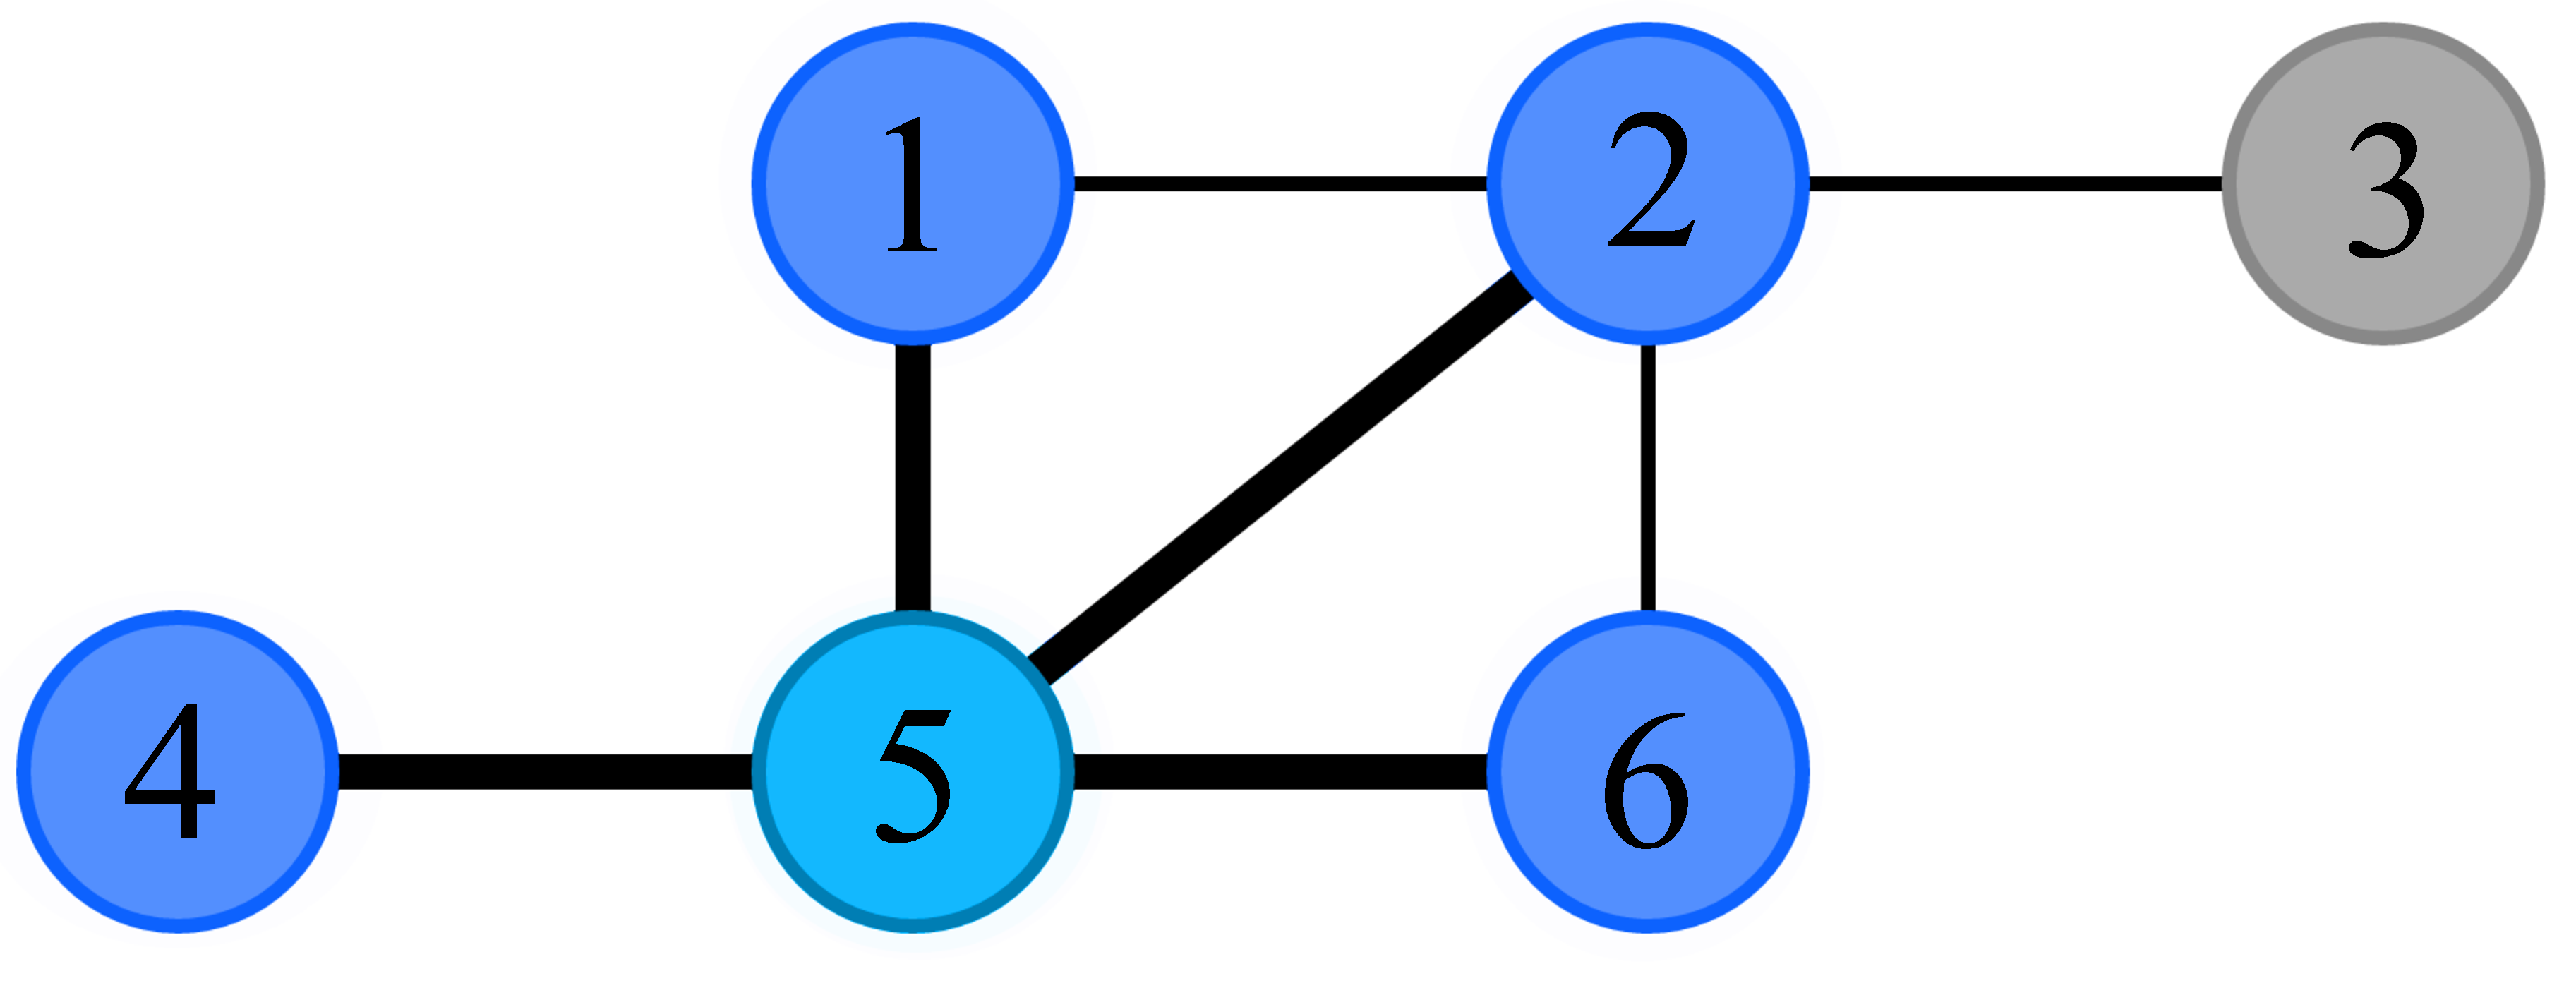
\includegraphics[width=8cm]{../figures/example-neighborhoods-2.pdf}
      \end{textblock*}
    }

    \vspace{4cm}

    \vfill

    \begin{itemize}
      \item<1-4> A \textbf{graph} is the set of vertices \emph{V} and a set of edges \emph{E}.
      \item<2-4> The \textbf{neighborhood} of a vertex $v$ is a set of all vertices adjacent to $v$ plus $v$ itself.
      \only<1-2>{\item<3> Example: The neighborhood of vertex 1: $\{1, 2, 5\}$.}
      \only<3>{\item<3> Example: The neighborhood of vertex 1: $\{1, 2, 5\}$.}
      \only<4>{\item<4> Example: The neighborhood of vertex 5: $\{1, 2, 4, 5, 6\}$.}
    \end{itemize}

  \end{frame}

  \subsection{Graph Coloring}

  \begin{frame}
    \frametitle{Vertex Coloring}

    \begin{textblock*}{\examplewidth}(0cm,\exampleheight) % {block width} (coords)
      \centering
      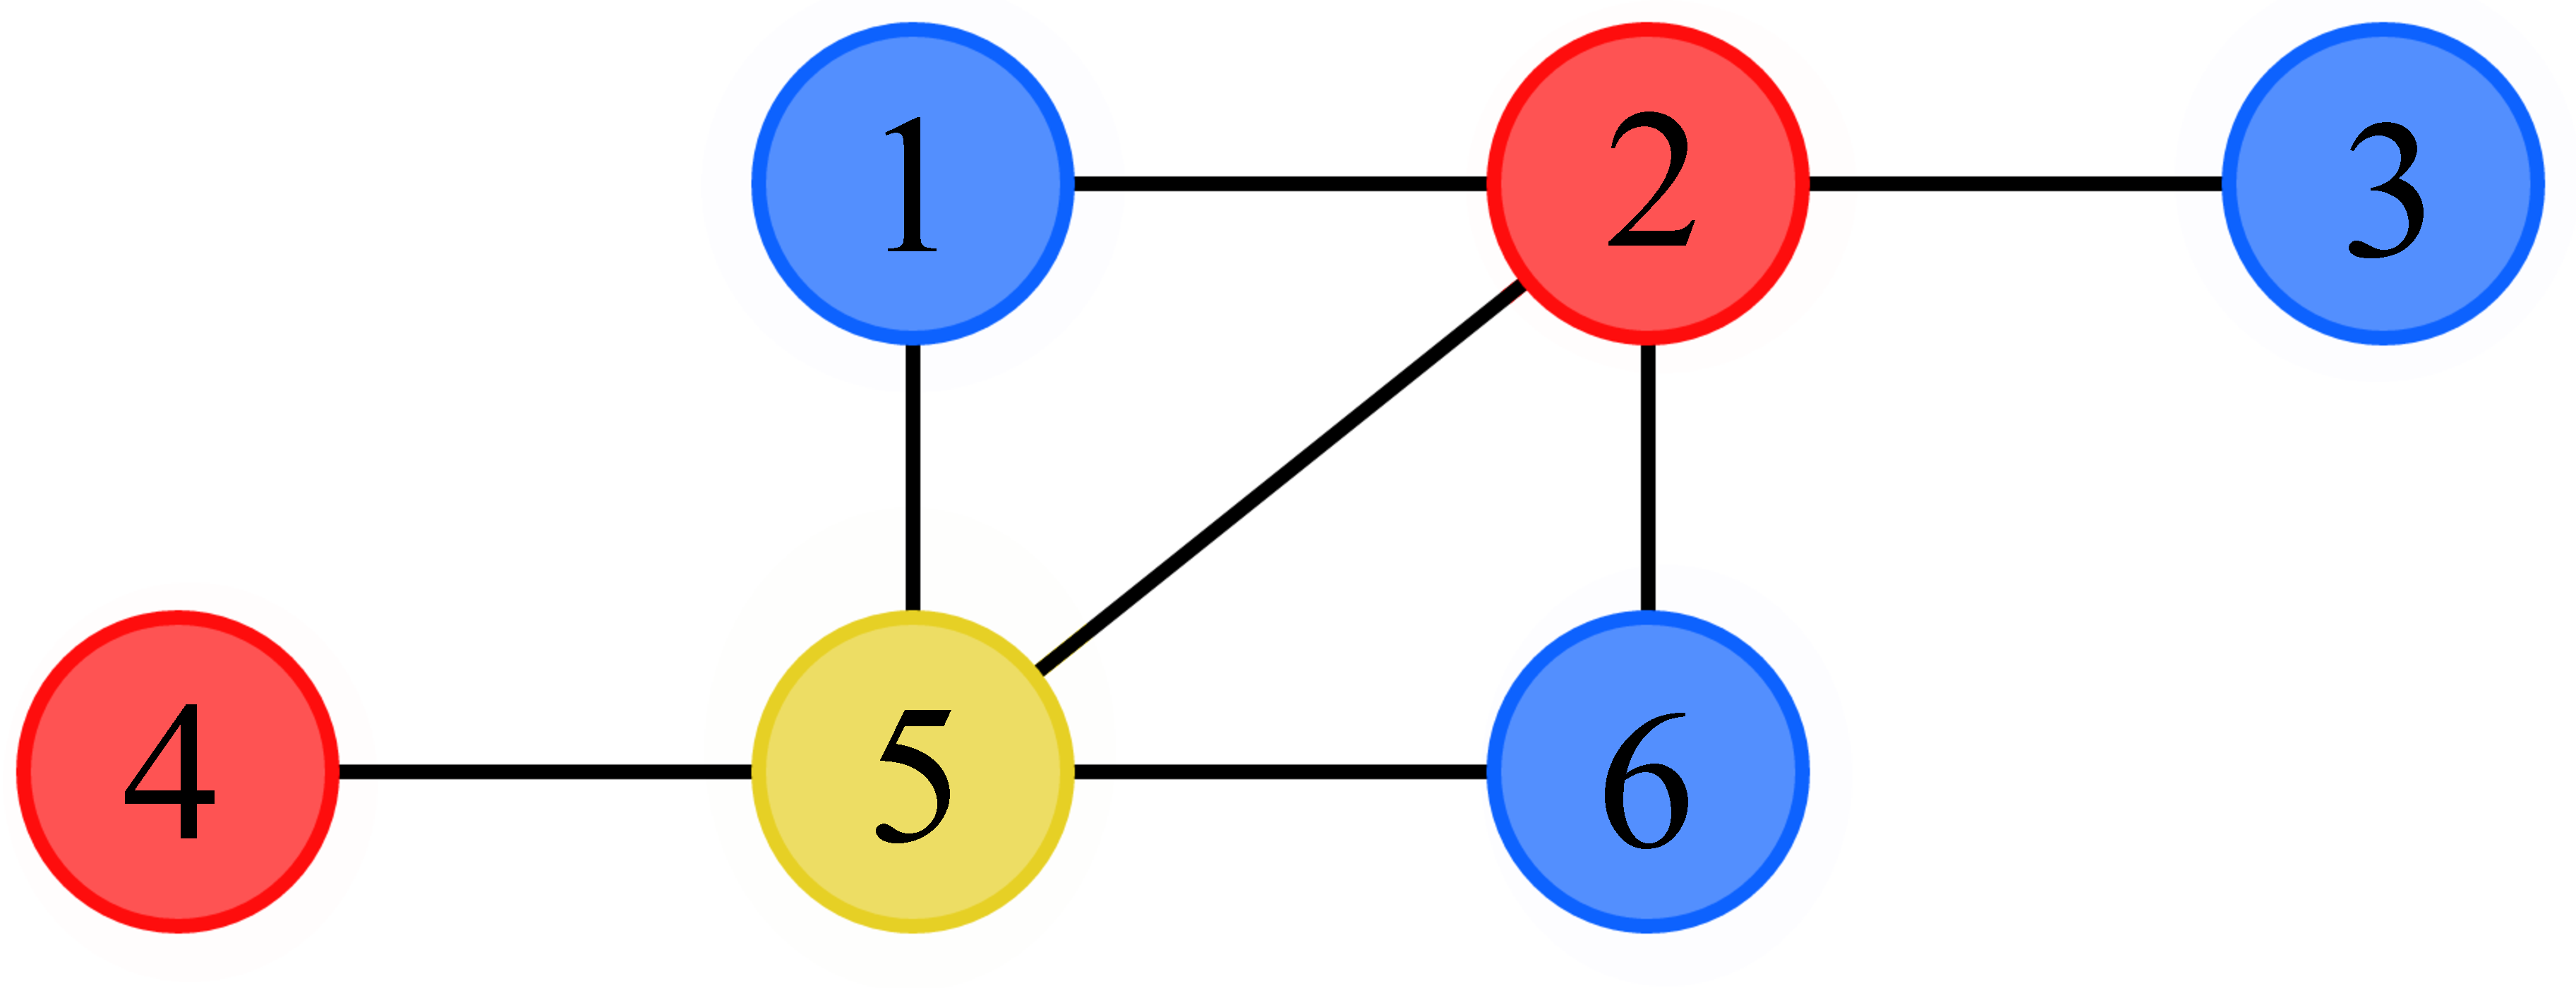
\includegraphics[width=8cm]{../figures/example-vcp.pdf}
    \end{textblock*}

    \vspace{4cm}

    \vfill


    \begin{itemize}
      \item A proper \textbf{vertex coloring} of a graph $G$ is an assignment of colors to each vertex such that no adjacent vertices share the same color.
      \item The \textbf{chromatic number} of $G$ is the minimum number of colors needed to properly color $G$.
    \end{itemize}
  \end{frame}

  \begin{frame}
    \frametitle{Conflict-Free Coloring}

    \begin{figure}[h]
      \centering
      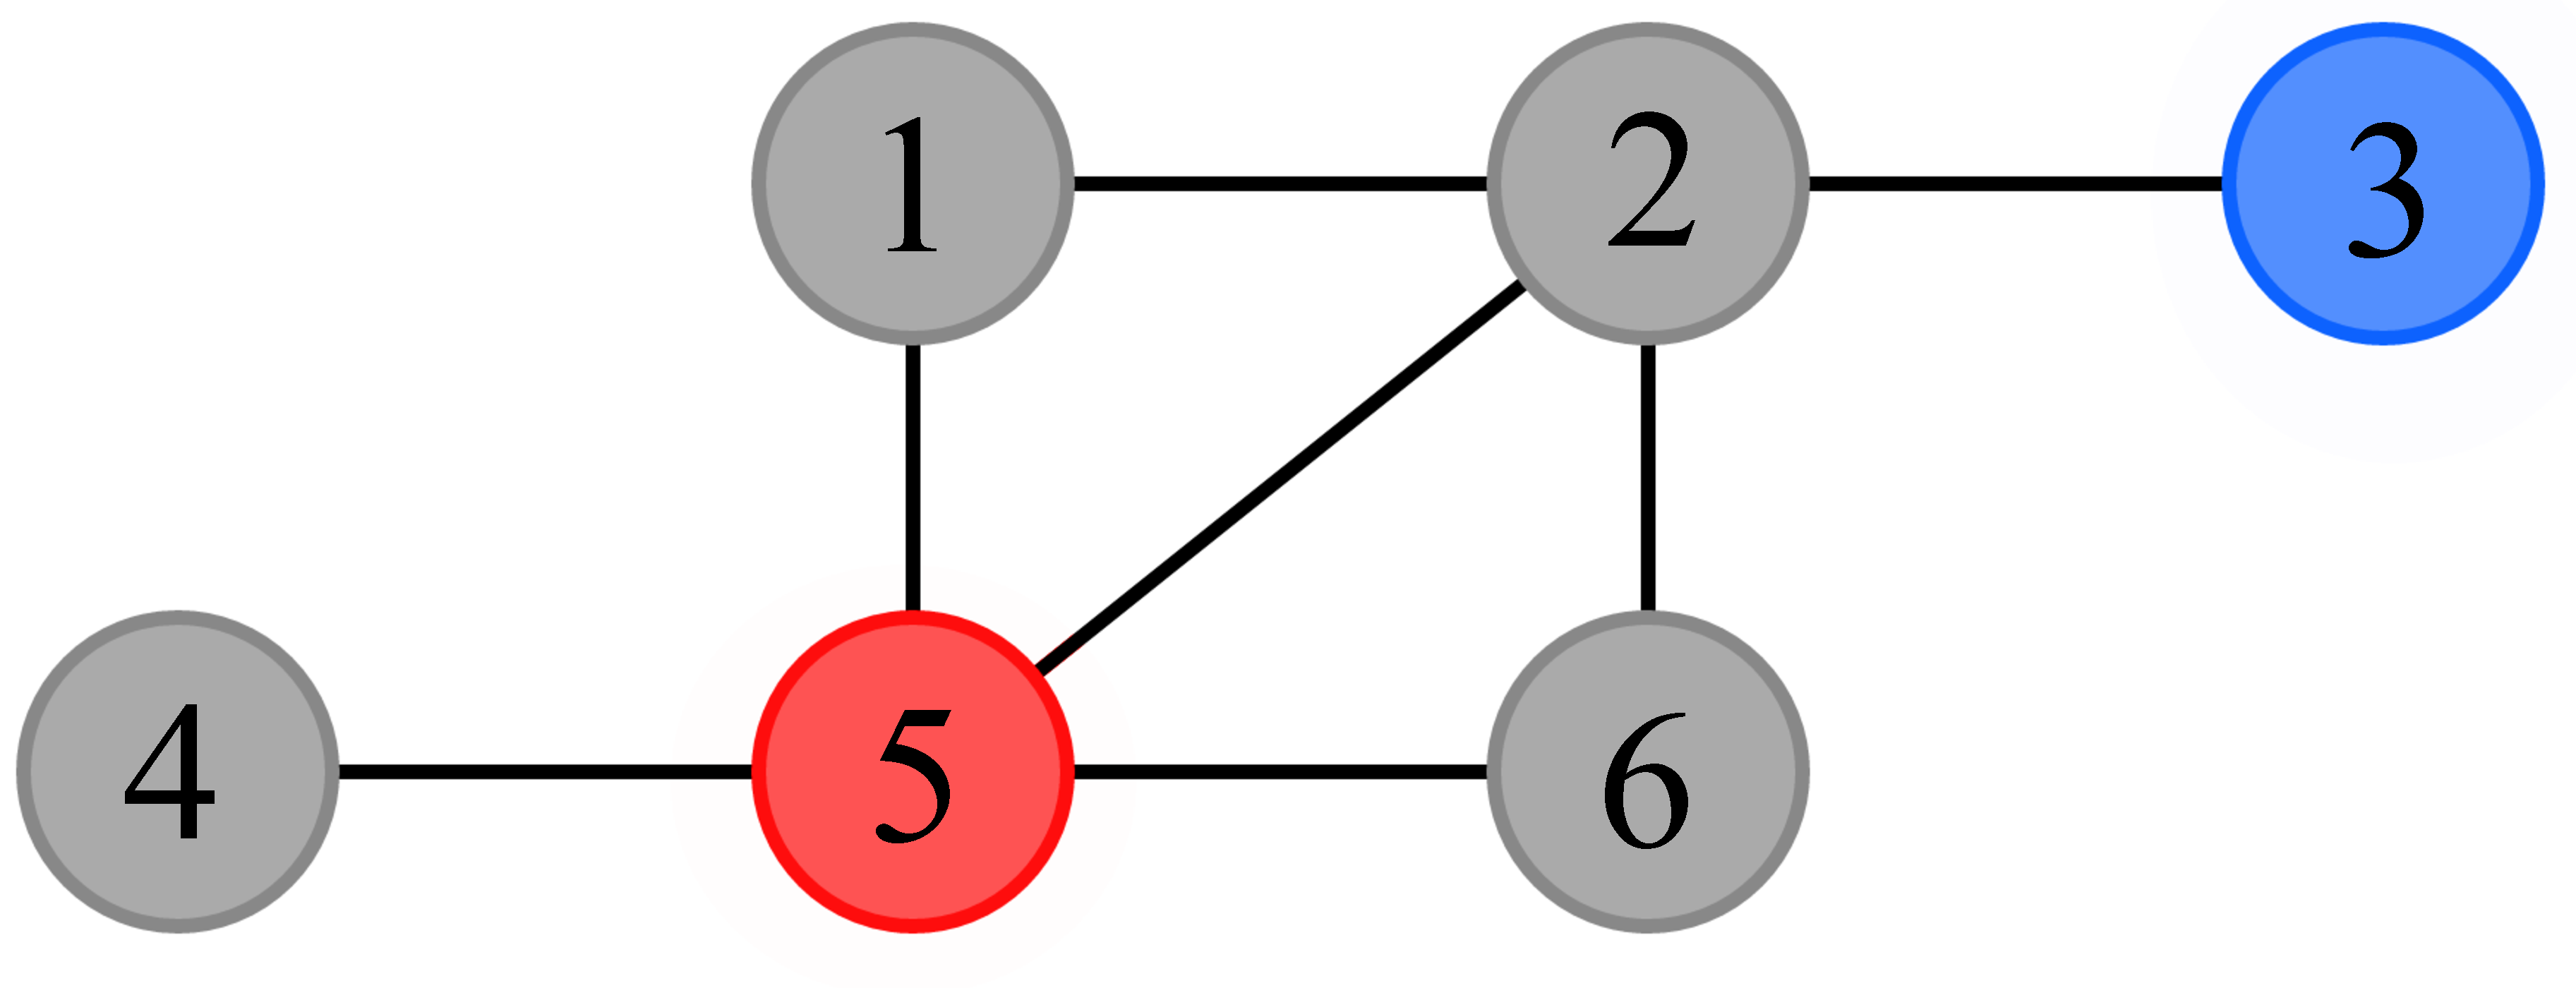
\includegraphics[width=8cm]{../figures/example-cfcp.pdf}
    \end{figure}


    \begin{itemize}
      \item A \textbf{conflict-free coloring} of a graph $G$ assigns colors to some vertices such that there is a uniquely colored vertex within the closed neighborhood of every vertex.
      \item Every proper vertex coloring of $G$ is also a conflict-free coloring of $G$. This is because every vertex can be its own conflict-free neighbor.
    \end{itemize}
  \end{frame}

  \addtocontents{toc}{\protect\vspace{14pt}}

  \section{Applications}

  \subsection{Wireless Networks}

  \subsection{RFID Networks}

  \addtocontents{toc}{\newpage}


  \section{CF Coloring for General Graphs}

  \section{CF Coloring for Planar Graphs}

  \begin{frame}[standout]
    \centering
    {Thanks to Peter Dolan, Elena Machkasova,

    and Peh Ng for their advice and feedback.}
    \vfill
    \href{https://github.com/devshawn/senior-seminar}{github.com/devshawn/senior-seminar}
    \vfill
    \ccbyncsa{}
  \end{frame}

\end{document}
